\chapter{準備}
\label{ch:seminar-00}

\begin{definition}{冪集合}{sem-power-set}
  集合 $\Omega$ に対し，$\Omega$ の部分集合全体を
  \[
    2^{\Omega} \defeq \{A \mid A \subset \Omega\}
  \]
  と書き，$\Omega$ の\textbf{冪集合}という．
\end{definition}

%% ============================================================
%% 位相空間
%% ============================================================
\section{位相空間}
\label{sec:sem-topology}

\begin{definition}{位相空間}{sem-topological-space}
  集合 $\Omega$ と部分集合族 $\mathcal{O} \subset 2^{\Omega}$ の組
  $(\Omega, \mathcal{O})$ が\textbf{位相空間}であるとは，
  次の3条件を満たすことをいう：
  \begin{enumerate}
    \item[(i)] $\emptyset, \Omega \in \mathcal{O}$，
    \item[(ii)] $U_1, \ldots, U_n \in \mathcal{O} \Longrightarrow
      \bigcap_{k=1}^{n} U_k \in \mathcal{O}$（有限交叉で閉じる），
    \item[(iii)] $\{U_\lambda\}_{\lambda \in \Lambda} \subset \mathcal{O}
      \Longrightarrow \bigcup_{\lambda \in \Lambda} U_\lambda \in \mathcal{O}$
      （任意濃度の和集合で閉じる）．
  \end{enumerate}
  $\mathcal{O}$ の元を\textbf{開集合}，$\mathcal{O}$ を $\Omega$ 上の\textbf{位相}という．
  ある開集合 $U \in \mathcal{O}$ を用いて $F = \Omega \setminus U$ と書ける
  $F \subset \Omega$ を\textbf{閉集合}という．
\end{definition}

\begin{definition}{稠密集合}{sem-dense}
  位相空間 $(\Omega, \mathcal{O})$ の部分集合 $D \subset \Omega$ が\textbf{稠密}とは，
  任意の空でない開集合 $U \in \mathcal{O}$ に対して $D \cap U \neq \emptyset$
  となることをいう．
\end{definition}

\begin{definition}{可分性}{sem-separable}
  位相空間 $(\Omega, \mathcal{O})$ が可算な稠密部分集合
  （定義~\ref{def:sem-dense}）をもつとき，
  $(\Omega, \mathcal{O})$ は\textbf{可分}であるという．
\end{definition}

\begin{figure}[H]
\centering
\begin{tikzpicture}[scale=1.0]
  %% 数直線 Ω = R
  \draw[thick, ->] (-0.5, 0) -- (8.0, 0);
  \node[right, font=\small] at (8.0, 0) {$\Omega = \R$};

  %% 可算稠密集合 D = {q_1, q_2, ...}：番号付けで可算性を強調
  %% 一部に番号を付ける
  \foreach \k/\xpos in {1/0.5, 2/2.0, 3/4.5, 4/6.5, 5/1.2, 6/3.3, 7/5.7, 8/7.4} {
    \fill[blue] (\xpos, 0) circle (1.5pt);
    \node[blue, font=\scriptsize, below] at (\xpos, -0.1) {$q_{\k}$};
  }
  %% 番号なしの追加点（無限に並ぶことを示唆）
  \foreach \xpos in {0.85, 1.7, 2.5, 2.85, 3.7, 4.1, 4.85, 5.3, 6.1, 6.85, 7.7} {
    \fill[blue!60] (\xpos, 0) circle (1pt);
  }

  %% 任意の点 x（無理数）と任意精度の近傍
  \fill[red] (4.7, 0) circle (2pt);
  \node[red, font=\small, above] at (4.7, 0.1) {$x$};
  %% ε-近傍を示す赤線
  \draw[red, thick]
    (4.45, 0.6) -- (4.45, 0.8) -- (4.95, 0.8) -- (4.95, 0.6)
    node[above, font=\footnotesize, midway] at (4.7, 0.85) {$\varepsilon$ 近傍};

  %% 近傍内の D の点（近似列の存在）
  \draw[->, thick, blue!50!green]
    (4.6, 0.1) -- (4.6, 0.6);
  \node[blue!50!green, font=\footnotesize, anchor=west] at (5.05, 0.7)
    {$\exists q_k \in D,\; d(x, q_k) < \varepsilon$};

  %% 凡例
  \node[blue, font=\footnotesize, anchor=west] at (-0.3, -0.7)
    {$D = \{q_1, q_2, \ldots\}$ は可算（番号付けできる）};
  \node[font=\footnotesize, anchor=west] at (-0.3, -1.05)
    {かつ稠密（任意の $x$ を任意精度で近似）};
\end{tikzpicture}
\caption{可分性のイメージ（$\Q \subset \R$ を例に）．
青点 $D = \{q_1, q_2, \ldots\}$ は可算（番号付け可能）．
さらに任意の点 $x \in \R$ と任意の精度 $\varepsilon > 0$ に対し
$d(x, q_k) < \varepsilon$ をみたす $q_k$ がとれる（稠密）．
可算性と稠密性の両立が可分性の本質．}
\label{fig:sem-dense-separable}
\end{figure}

%% ============================================================
%% 距離空間
%% ============================================================
\section{距離空間}
\label{sec:sem-metric-space}

\begin{definition}{距離空間}{sem-metric-space}
  集合 $\Omega$ と関数 $d \colon \Omega \times \Omega \to [0, \infty)$ の組
  $(\Omega, d)$ が\textbf{距離空間}であるとは，
  次の3条件がすべての $x, y, z \in \Omega$ に対して成り立つことをいう：
  \begin{enumerate}
    \item[(i)] 同一性：$d(x, y) = 0 \iff x = y$，
    \item[(ii)] 対称性：$d(x, y) = d(y, x)$，
    \item[(iii)] 三角不等式：$d(x, z) \leq d(x, y) + d(y, z)$．
  \end{enumerate}
  関数 $d$ を $\Omega$ 上の\textbf{距離関数}という．
\end{definition}

\begin{definition}{ノルム空間}{sem-normed-space}
  実ベクトル空間 $V$ と関数 $\|\cdot\| \colon V \to [0, \infty)$ の組
  $(V, \|\cdot\|)$ が\textbf{ノルム空間}であるとは，
  次の3条件がすべての $x, y \in V$ と $\lambda \in \R$ に対して
  成り立つことをいう：
  \begin{enumerate}
    \item[(i)] 正定値性：$\|x\| = 0 \iff x = 0$，
    \item[(ii)] 斉次性：$\|\lambda x\| = |\lambda|\,\|x\|$，
    \item[(iii)] 三角不等式：$\|x + y\| \leq \|x\| + \|y\|$．
  \end{enumerate}
  関数 $\|\cdot\|$ を $V$ 上の\textbf{ノルム}という．
  ノルム空間は $d(x, y) \defeq \|x - y\|$ により
  距離空間（定義~\ref{def:sem-metric-space}）となる．
  $V$ が有限次元のとき，$(V, \|\cdot\|)$ を
  \textbf{有限次元ノルム空間}という．
  例えば $\R^n$ や $\R^{n \times m}$ はユークリッドノルム（フロベニウスノルム）により
  有限次元ノルム空間となる．
\end{definition}

\begin{definition}{開球}{sem-open-ball}
  距離空間 $(\Omega, d)$ 上の点 $x \in \Omega$ と半径 $r \in \R_{++}$ に対して，
  中心 $x$，半径 $r$ の\textbf{開球}を
  \[
    B_r(x) \defeq \{y \in \Omega \mid d(x, y) < r\}
  \]
  で定める．
\end{definition}

距離空間 $(\Omega, d)$ における開集合（定義~\ref{def:sem-topological-space}）は，
開球 $B_r(x)$ を用いて次のように特徴付けられる：
$U \subset \Omega$ が開集合であるとは，任意の $x \in U$ に対し
$B_r(x) \subset U$ をみたす $r \in \R_{++}$ が存在することをいう．

\begin{figure}[H]
\centering
\begin{tikzpicture}[scale=1.0]
  %% --- 左：開集合 U（境界は U に含まれない） ---
  \begin{scope}
    \node[above, font=\small\bfseries] at (1.7, 3.0) {開集合の例};
    %% U の領域（境界を点線で示し，「境界は含まない」）
    \draw[blue, dashed, thick, fill=blue!8]
      plot[smooth cycle, tension=0.7]
      coordinates {(0.2, 1.0) (0.7, 2.4) (2.1, 2.7) (3.2, 2.0)
                   (3.0, 0.8) (1.8, 0.2) (0.6, 0.4)};
    \node[blue, font=\small] at (1.9, 1.5) {$U$};

    %% 内点 x_1 とその開球
    \fill[red] (1.2, 1.7) circle (1.5pt);
    \node[red, font=\small, above right] at (1.2, 1.7) {$x_1$};
    \draw[red, thick] (1.2, 1.7) circle (0.35);
    \node[red, font=\footnotesize] at (1.2, 1.05) {$B_{r_1}(x_1) \subset U$};

    %% 内点 x_2 とその開球（境界に近い）
    \fill[red] (2.6, 2.0) circle (1.5pt);
    \node[red, font=\small, above] at (2.6, 2.05) {$x_2$};
    \draw[red, thick] (2.6, 2.0) circle (0.18);

    \node[font=\footnotesize, anchor=north] at (1.7, -0.1)
      {任意の点 $x \in U$ で $B_r(x) \subset U$ なる $r$ がとれる};
  \end{scope}

  %% --- 右：開集合でない例（境界点を含む） ---
  \begin{scope}[xshift=6.0cm]
    \node[above, font=\small\bfseries] at (1.7, 3.0) {開集合でない例};
    %% F の領域（境界を実線で示し，「境界も含む」）
    \draw[red!70!black, thick, fill=red!8]
      plot[smooth cycle, tension=0.7]
      coordinates {(0.2, 1.0) (0.7, 2.4) (2.1, 2.7) (3.2, 2.0)
                   (3.0, 0.8) (1.8, 0.2) (0.6, 0.4)};
    \node[red!70!black, font=\small] at (1.9, 1.5) {$F$};

    %% 境界上の点 x_0
    \fill[red] (3.18, 1.7) circle (1.5pt);
    \node[red, font=\small, right] at (3.22, 1.7) {$x_0$};
    %% B_r(x_0) が F からはみ出す様子
    \draw[red, thick, dashed] (3.18, 1.7) circle (0.4);
    \node[red, font=\footnotesize] at (3.6, 1.05) {$B_r(x_0) \not\subset F$};

    \node[font=\footnotesize, anchor=north] at (1.7, -0.1)
      {境界点 $x_0$ で $B_r(x_0)$ が外にはみ出す};
  \end{scope}
\end{tikzpicture}
\caption{開集合の概念図．左：$U$ は開集合で，任意の点 $x \in U$ について
十分小さい開球 $B_r(x)$ が $U$ に含まれる（境界は $U$ に含まれない；点線で表示）．
右：$F$ は境界を含むため開集合でなく，境界点 $x_0$ ではどんなに $r$ を
小さくしても $B_r(x_0) \not\subset F$．
$\Omega$ 上の開集合全体が位相 $\mathcal{O}_d$ をなす．}
\label{fig:sem-open-set}
\end{figure}

\begin{definition}{収束列}{sem-convergence}
  距離空間 $(\Omega, d)$ における列 $(x_n)_{n \geq 1} \subset \Omega$ が
  点 $x \in \Omega$ に\textbf{収束}するとは，
  任意の $\varepsilon > 0$ に対してある $N \in \N$ が存在して
  $n \geq N \Longrightarrow d(x_n, x) < \varepsilon$ となることをいう．
  このとき $\lim_{n \to \infty} x_n = x$ または $x_n \to x$ と書く．
\end{definition}

\begin{definition}{完備性}{sem-complete-metric}
  距離空間 $(\Omega, d)$ の列 $(x_n)_{n \geq 1} \subset \Omega$ が
  \textbf{Cauchy 列}であるとは，
  任意の $\varepsilon > 0$ に対してある $N \in \N$ が存在して
  $n, m \geq N \Longrightarrow d(x_n, x_m) < \varepsilon$ となることをいう．
  $(\Omega, d)$ が\textbf{完備}であるとは，
  $\Omega$ における任意の Cauchy 列が $\Omega$ の点に収束する
  （定義~\ref{def:sem-convergence}）ことをいう．すなわち
  \[
    \forall (x_n)_{n \geq 1} \subset \Omega \text{ Cauchy 列},\;
    \exists x \in \Omega,\;
    x_n \to x.
  \]
  収束の定義に展開すれば
  \[
    \forall (x_n)_{n \geq 1} \subset \Omega \text{ Cauchy 列},\;
    \exists x \in \Omega,\;
    \forall \varepsilon > 0,\;
    \exists N \in \N,\;
    n \geq N \Longrightarrow d(x_n, x) < \varepsilon.
  \]
\end{definition}

\begin{figure}[H]
\centering
\begin{tikzpicture}[scale=1.0]
  %% --- 左：完備な空間 Ω = [0, 4] ---
  \begin{scope}
    \node[above, font=\small\bfseries] at (2.2, 1.7) {完備：$\Omega = [0, 4]$};
    \draw[thick] (0, 1.0) -- (4.2, 1.0);
    \fill[black] (0, 1.0) circle (1.5pt);
    \fill[black] (4.2, 1.0) circle (1.5pt);

    %% Cauchy sequence x_k = 1/k * 3 (decreasing toward 0)
    \foreach \k/\xpos in {1/3.0, 2/1.5, 3/1.0, 4/0.75, 5/0.6, 6/0.5} {
      \fill[blue] (\xpos, 1.0) circle (1.5pt);
    }
    \node[blue, font=\scriptsize, above] at (3.0, 1.1) {$x_1$};
    \node[blue, font=\scriptsize, above] at (1.5, 1.1) {$x_2$};
    \node[blue, font=\scriptsize, above] at (1.0, 1.1) {$x_3$};
    \node[blue, font=\footnotesize, above] at (0.5, 1.3) {$\cdots$};

    %% limit point at 0 ∈ Ω
    \fill[red] (0, 1.0) circle (2.5pt);
    \node[red, font=\small, below] at (0, 0.85) {$x^*$};
    \node[red, font=\footnotesize, below] at (0, 0.5) {$\in \Omega$};

    %% convergence arrow
    \draw[->, gray, thick]
      (1.0, 0.45) .. controls (0.5, 0.5) .. (0.05, 0.95);
    \node[font=\footnotesize, gray, anchor=west] at (1.1, 0.4) {収束先};
  \end{scope}

  %% --- 右：完備でない $\Omega' = (0, 4]$ ---
  \begin{scope}[xshift=5.5cm]
    \node[above, font=\small\bfseries] at (2.2, 1.7) {完備でない：$\Omega' = (0, 4]$};
    \draw[thick] (0.05, 1.0) -- (4.2, 1.0);
    %% 0 を除く: open endpoint
    \draw[thick, fill=white] (0, 1.0) circle (2.0pt);
    \fill[black] (4.2, 1.0) circle (1.5pt);

    %% same Cauchy 列
    \foreach \xpos in {3.0, 1.5, 1.0, 0.75, 0.6, 0.5} {
      \fill[blue] (\xpos, 1.0) circle (1.5pt);
    }

    %% 極限が Ω' の外
    \draw[red, very thick] (-0.18, 0.83) -- (0.18, 1.17);
    \draw[red, very thick] (-0.18, 1.17) -- (0.18, 0.83);
    \node[red, font=\small, below] at (0, 0.7) {$x^*$};
    \node[red, font=\footnotesize, below] at (0, 0.4) {$\notin \Omega'$};
  \end{scope}
\end{tikzpicture}
\caption{完備性の概念．Cauchy 列 $(x_k)$ は項間距離が無限小に縮まる
（$\forall \varepsilon > 0,\; \exists N,\; k, l \geq N \Rightarrow d(x_k, x_l) < \varepsilon$）．
左：完備な $\Omega$ では極限 $x^*$ が $\Omega$ 内に存在し $x_k \to x^*$．
右：$\Omega' = (0, 4]$（端点 $0$ を除外）では同じ Cauchy 列の極限 $0$ が
$\Omega'$ の外に逃げ，完備でない．}
\label{fig:sem-completeness}
\end{figure}

\begin{definition}{Polish 空間}{sem-polish}
  完備かつ可分な距離空間を\textbf{Polish 空間}という．
  例：$\R^d$ はユークリッド距離に関して Polish 空間である
  （$\Q^d$ が可算稠密部分集合を与える）．
\end{definition}

\begin{figure}[H]
\centering
\begin{tikzpicture}[scale=1.0]
  %% Ω = R
  \draw[thick, ->] (-0.5, 0) -- (8.0, 0);
  \node[right, font=\small] at (8.0, 0) {$\R$};

  %% Q = countable dense subset, labeled
  %% spread Q points; some near limit x* = π
  \foreach \k/\xpos in {1/0.5, 2/1.5, 3/4.0, 4/6.5, 5/7.3} {
    \fill[blue] (\xpos, 0) circle (1.5pt);
    \node[blue, font=\scriptsize, below] at (\xpos, -0.15) {$q_{\k}$};
  }
  %% Cauchy subsequence (q_{k_n}) → x* (irrational point)
  \def\xstar{3.14}
  \foreach \i/\xpos/\lab in {6/2.5/$q_{k_1}$, 7/3.0/$q_{k_2}$, 8/3.13/$q_{k_3}$} {
    \fill[blue] (\xpos, 0) circle (1.5pt);
    \node[blue, font=\scriptsize, above] at (\xpos, 0.1) {\lab};
  }
  %% extra Q points (background density)
  \foreach \xpos in {1.0, 1.9, 4.5, 5.0, 5.5, 6.0, 6.9, 7.6} {
    \fill[blue!50] (\xpos, 0) circle (1pt);
  }

  %% x* (limit, irrational) in R
  \fill[red] (\xstar, 0) circle (2.5pt);
  \node[red, font=\small, above] at (\xstar, 0.3) {$x^*$};
  \node[red, font=\scriptsize] at (\xstar, 0.6) {（無理数）};

  %% arrow from Cauchy seq to x*
  \draw[->, blue!50!green, thick]
    (2.7, 1.3) .. controls (3.0, 1.0) .. (\xstar, 0.4);
  \node[blue!50!green, font=\footnotesize, anchor=south west] at (1.3, 1.25)
    {Cauchy 列 $(q_{k_n}) \to x^*$};

  %% labels
  \node[font=\footnotesize, anchor=west, blue] at (-0.3, -1.0)
    {\textbf{可分性}：可算稠密な $\Q = \{q_1, q_2, \ldots\} \subset \R$};
  \node[font=\footnotesize, anchor=west, red!70!black] at (-0.3, -1.4)
    {\textbf{完備性}：Cauchy 列の極限 $x^*$ が $\R$ 内に存在
      （無理数も $\R$ には含まれる）};
\end{tikzpicture}
\caption{Polish 空間（完備可分距離空間）のイメージ．代表例 $\R$ 上で：
$\Q$ は可算かつ稠密（可分性）．
$\Q$ 内の Cauchy 列 $(q_{k_n})$ の極限は無理数になりうるが，
それも $\R$ 内に存在する（完備性）．
$\Q$ 自身は完備でない（極限を $\Q$ に拾えない）が，
$\R$ はその「完備化」として機能する．}
\label{fig:sem-polish}
\end{figure}

\begin{definition}{連続写像}{sem-continuous}
  距離空間 $(\Omega_1, d_1)$，$(\Omega_2, d_2)$ の間の写像
  $f \colon \Omega_1 \to \Omega_2$ が点 $x \in \Omega_1$ で\textbf{連続}であるとは，
  \[
    \forall \varepsilon > 0,\; \exists \delta > 0,\;
    d_1(x, y) < \delta \Longrightarrow d_2(f(x), f(y)) < \varepsilon
  \]
  が成り立つことをいう．$f$ が $\Omega_1$ の全点で連続であるとき，
  $f$ は\textbf{連続写像}であるという．
  同値な条件として，$\Omega_1$ の任意の収束列 $x_n \to x$ に対して
  $f(x_n) \to f(x)$ が成り立つことが挙げられる．
\end{definition}

\begin{proposition}{連続写像による閉集合の逆像}{sem-preimage-closed}
  距離空間 $(\Omega_1, d_1)$，$(\Omega_2, d_2)$ の間の連続写像
  $f \colon \Omega_1 \to \Omega_2$（定義~\ref{def:sem-continuous}）に対して，
  $F \subset \Omega_2$ が閉集合ならば $f^{-1}(F)$ も閉集合である．
\end{proposition}

\begin{proof}
  $f^{-1}(F)$ の任意の収束列 $(x_n)$ をとり，極限を $x^*$ とする．
  $f(x_n) \in F$ であり，$f$ の連続性から $f(x_n) \to f(x^*)$．
  $F$ は閉集合だから $f(x^*) \in F$，すなわち $x^* \in f^{-1}(F)$．
  ゆえに $f^{-1}(F)$ は閉集合．
\end{proof}

\begin{definition}{有界集合}{sem-bounded}
  $\R^n$ の部分集合 $S \subset \R^n$ が\textbf{有界}であるとは，
  ある $M > 0$ が存在して
  \[
    \forall x \in S,\quad \|x\| \leq M
  \]
  が成り立つことをいう．ここで $\|\cdot\|$ はユークリッドノルムを表す．
\end{definition}

\begin{definition}{コンパクト集合}{sem-compact}
  距離空間 $(\Omega, d)$ の部分集合 $K \subset \Omega$ が
  \textbf{コンパクト}であるとは，
  $K$ における任意の点列 $(x_n)_{n \geq 1}$ が，
  $K$ の点に収束する部分列 $(x_{n_k})_{k \geq 1}$ を持つことをいう
  （列コンパクト性）．
\end{definition}

\begin{claim}{Bolzano-Weierstrass の定理}{sem-bolzano-weierstrass}
  $\R^n$ における任意の有界列 $(x_n)_{n \geq 1} \subset \R^n$ は，
  収束する部分列 $(x_{n_k})_{k \geq 1}$ を持つ．
\end{claim}

\begin{theorem}{Heine-Borel の定理}{sem-heine-borel}
  $\R^n$ の部分集合 $K \subset \R^n$ に対して，
  次の2条件は同値である：
  \begin{enumerate}
    \item[(i)] $K$ はコンパクト（定義~\ref{def:sem-compact}）である．
    \item[(ii)] $K$ は閉集合（定義~\ref{def:sem-topological-space}）かつ
      有界（定義~\ref{def:sem-bounded}）である．
  \end{enumerate}
\end{theorem}

\begin{proof}
  \textbf{(i) $\Rightarrow$ (ii)：コンパクト $\Rightarrow$ 有界かつ閉．}

  \textit{有界性．}
  $K$ が有界でないと仮定する．すると各 $n \in \N$ に対して
  $\|x_n\| > n$ をみたす $x_n \in K$ が存在する．
  $K$ のコンパクト性より $(x_n)$ はある収束部分列 $(x_{n_k})$ を持ち，
  その極限 $x^* \in K$ について $\|x_{n_k}\| \to \|x^*\|$．
  一方 $\|x_{n_k}\| > n_k \to \infty$ であり矛盾．
  ゆえに $K$ は有界．

  \textit{閉性．}
  $K$ への収束列 $(x_n)$ を任意にとり，極限を $x^*$ とする（$x^* \in \R^n$）．
  $K$ のコンパクト性より $(x_n)$ はある収束部分列 $(x_{n_k})$ を持ち，
  その極限 $y^* \in K$ が存在する．
  部分列も元の列の収束先と同じ極限を持つから $y^* = x^*$，
  すなわち $x^* \in K$．ゆえに $K$ は閉集合．

  \textbf{(ii) $\Rightarrow$ (i)：有界かつ閉 $\Rightarrow$ コンパクト．}

  $K$ の任意の点列 $(x_n)$ をとる．
  $K$ は有界ゆえ $(x_n)$ は $\R^n$ における有界列である．
  Bolzano-Weierstrass の定理（主張~\ref{clm:sem-bolzano-weierstrass}）より
  $(x_n)$ はある収束部分列 $(x_{n_k})$ を持ち，その極限を $x^* \in \R^n$ とする．
  $x_{n_k} \in K$ かつ $K$ は閉集合だから $x^* \in K$．
  ゆえに $K$ はコンパクト．
\end{proof}

\begin{theorem}{Weierstrass の最大値の定理}{sem-weierstrass}
  $K \subset \R^n$ を空でないコンパクト集合，
  $f \colon K \to \R$ を連続関数（定義~\ref{def:sem-continuous}）とする．
  このとき $f$ は $K$ 上で最小値および最大値を達成する，すなわち
  \[
    \exists x^* \in K,\quad f(x^*) = \min_{x \in K} f(x).
  \]
\end{theorem}

\begin{proof}
  最小値について示す（最大値は $-f$ に適用すればよい）．

  $p^* \defeq \inf_{x \in K} f(x) \in [-\infty, +\infty)$ とおく．
  下限の定義より，各 $n \in \N$ に対して
  \[
    f(x_n) < p^* + \tfrac{1}{n}
  \]
  をみたす $x_n \in K$ が存在する（最小化列）．
  $K$ のコンパクト性より $(x_n)$ はある収束部分列 $(x_{n_k})$ を持ち，
  極限 $x^* \in K$ が存在する．
  $f$ の連続性（定義~\ref{def:sem-continuous}）より
  \[
    f(x^*) = \lim_{k \to \infty} f(x_{n_k}) = p^*.
  \]
  特に $p^* = f(x^*) \in \R$ であり，最小値は $x^*$ で達成される．
\end{proof}

\begin{proposition}{有限次元ノルム空間上の線形関数の連続性}{sem-finite-dim-linear-continuous}
  有限次元ノルム空間 $V$ 上の任意の線形関数 $f \colon V \to \R$ は連続である．
\end{proposition}

%% ============================================================
%% 測度論
%% ============================================================
\section{測度論}
\label{sec:sem-measure-theory}

\subsection{可測空間と確率測度}
\label{sec:sem-measurable}

\begin{definition}{$\sigma$-代数}{sem-sigma-algebra}
  集合 $\Omega$ の部分集合族 $\mathcal{F} \subset 2^{\Omega}$ が
  \textbf{$\sigma$-代数}であるとは，
  以下の3条件を満たすことをいう：
  \begin{enumerate}
    \item[(i)] $\Omega \in \mathcal{F}$，
    \item[(ii)] $A \in \mathcal{F} \Longrightarrow A^c \in \mathcal{F}$（補集合で閉じる），
    \item[(iii)] $A_1, A_2, \ldots \in \mathcal{F} \Longrightarrow
      \bigcup_{k=1}^{\infty} A_k \in \mathcal{F}$（可算合併で閉じる）．
  \end{enumerate}
\end{definition}

\begin{definition}{可測空間}{sem-measurable-space}
  集合 $\Omega$ と $\Omega$ 上の $\sigma$-代数 $\mathcal{F}$ の組
  $(\Omega, \mathcal{F})$ を\textbf{可測空間}という．
  $\mathcal{F}$ の元を\textbf{可測集合}という．
\end{definition}

\begin{definition}{可測写像}{sem-measurable-map}
  可測空間 $(\Omega_1, \mathcal{F}_1)$ から $(\Omega_2, \mathcal{F}_2)$ への
  写像 $T \colon \Omega_1 \to \Omega_2$ が\textbf{可測}であるとは，
  $T^{-1}(A) \in \mathcal{F}_1$ がすべての $A \in \mathcal{F}_2$ に対して成り立つことをいう．
\end{definition}

\begin{definition}{ボレル $\sigma$-代数}{sem-borel}
  位相空間 $(\Omega, \mathcal{O})$ のすべての開集合
  （定義~\ref{def:sem-topological-space}）
  を含む最小の $\sigma$-代数を
  \textbf{ボレル $\sigma$-代数}といい，$\Bb(\Omega)$ と記す．
\end{definition}

\begin{definition}{可測関数}{sem-measurable-function}
  可測空間 $(\Omega, \mathcal{F})$ から $(\R, \Bb(\R))$ への可測写像
  $f \colon \Omega \to \R$（定義~\ref{def:sem-measurable-map}）を
  \textbf{可測関数}という．
  特に Polish 空間 $\X$ にボレル $\sigma$-代数 $\Bb(\X)$ を入れた
  可測空間上の可測関数を\textbf{ボレル可測関数}ともいう．
\end{definition}

\begin{definition}{積可測空間}{sem-product-measurable}
  距離空間 $(\X, d_\X)$, $(\Y, d_\Y)$ に対して，
  積空間 $\X \times \Y$ に\textbf{積距離}
  \[
    d\bigl((x, y), (x', y')\bigr) \defeq d_\X(x, x') + d_\Y(y, y')
  \]
  を入れたときのボレル $\sigma$-代数を $\Bb(\X \times \Y)$ と記し，
  可測空間 $(\X \times \Y, \Bb(\X \times \Y))$ を
  $(\X, \Bb(\X))$ と $(\Y, \Bb(\Y))$ の\textbf{積可測空間}という．
\end{definition}

\begin{definition}{射影}{sem-projection}
  距離空間 $\X$, $\Y$ の積空間 $\X \times \Y$
  （定義~\ref{def:sem-product-measurable}）に対して，
  \textbf{射影} $P_\X \colon \X \times \Y \to \X$，
  $P_\Y \colon \X \times \Y \to \Y$ を
  \[
    P_\X(x, y) \defeq x,
    \qquad
    P_\Y(x, y) \defeq y
  \]
  で定める．$P_\X$，$P_\Y$ はともに連続であり，可測写像
  （定義~\ref{def:sem-measurable-map}）でもある．
\end{definition}

\begin{definition}{測度}{sem-measure}
  可測空間 $(\Omega, \mathcal{F})$ 上の\textbf{測度}とは，
  関数 $\mu \colon \mathcal{F} \to [0, \infty]$ であって，
  次の 2 条件を満たすものをいう：
  \begin{enumerate}
    \item[(i)] $\mu(\emptyset) = 0$，
    \item[(ii)] 互いに素な可測集合 $A_1, A_2, \ldots \in \mathcal{F}$ に対して
      $\mu\bigl(\bigcup_{k=1}^{\infty} A_k\bigr) = \sum_{k=1}^{\infty} \mu(A_k)$
      （可算加法性）．
  \end{enumerate}
\end{definition}

\begin{definition}{確率測度}{sem-probability-measure}
  可測空間 $(\Omega, \mathcal{F})$ 上の測度 $\mu$ が $\mu(\Omega) = 1$ を満たすとき，
  $\mu$ を\textbf{確率測度}という．
  $\Omega$ 上の確率測度の全体を $\Mm_+^1(\Omega)$ と記す．
\end{definition}

\subsection{測度に対する積分}
\label{sec:sem-integration}

\begin{definition}{指示関数}{sem-indicator}
  集合 $\Omega$ の部分集合 $A \subset \Omega$ に対して，
  \textbf{指示関数} $\mathbf{1}_A \colon \Omega \to \{0, 1\}$ を
  \[
    \mathbf{1}_A(y) \defeq
    \begin{cases}
      1 & y \in A, \\
      0 & y \notin A
    \end{cases}
  \]
  で定める．
\end{definition}

\begin{definition}{単関数}{sem-simple-function}
  可測空間 $(\Omega, \mathcal{F})$ 上の関数 $s \colon \Omega \to \R_+$ が
  \textbf{単関数}であるとは，互いに素な可測集合
  $A_1, \ldots, A_m \in \mathcal{F}$ と非負定数 $c_1, \ldots, c_m \geq 0$ を用いて
  \[
    s = \sum_{k=1}^{m} c_k \mathbf{1}_{A_k}
  \]
  と表せることをいう．
\end{definition}

\begin{definition}{非負可測関数の積分}{sem-nonneg-integral}
  可測空間 $(\Omega, \mathcal{F})$ 上の測度 $\mu$ に対し，
  非負可測関数の積分を以下の 2 段階で定める：
  \begin{itemize}
    \item[(i)] 単関数 $s = \sum_{k=1}^{m} c_k \mathbf{1}_{A_k}$
      （定義~\ref{def:sem-simple-function}）の積分を
      \[
        \int_\Omega s \, \d\mu \defeq \sum_{k=1}^{m} c_k \, \mu(A_k)
      \]
      で定める．
    \item[(ii)] 非負可測関数 $f \colon \Omega \to [0, \infty]$ の積分を
      \[
        \int_\Omega f \, \d\mu \defeq
        \sup\!\left\{ \int_\Omega s \, \d\mu
        \;\middle|\; s \text{ は単関数}, \; 0 \leq s \leq f \right\}
      \]
      で定める．この値は常に $[0, +\infty]$ に存在し well-defined である．
  \end{itemize}
\end{definition}

\begin{proposition}{単調収束定理と単関数近似}{sem-mct}
  可測空間 $(\Omega, \mathcal{F})$ 上の測度 $\mu$ に対して次が成り立つ．
  \begin{enumerate}
    \item[(i)] \textbf{単関数近似}：任意の非負可測関数
      $f \colon \Omega \to [0, \infty]$ に対して，
      各点で $f_n \uparrow f$ を満たす単関数の単調増加列 $(f_n)_{n \geq 1}$ が存在する．
    \item[(ii)] \textbf{単調収束定理}：
      非負可測関数の単調増加列 $f_n \uparrow f$ に対して
      $\int f_n \, \d\mu \uparrow \int f \, \d\mu$．
  \end{enumerate}
\end{proposition}

\begin{proposition}{積分の測度に関する線形性}{sem-measure-linearity}
  可測空間 $(\Omega, \mathcal{F})$ 上の測度 $\mu_1, \ldots, \mu_n$，
  非負係数 $a_1, \ldots, a_n \geq 0$，および非負可測関数
  $f \colon \Omega \to [0, \infty]$ に対して，
  \[
    \int_\Omega f \, \d\!\Bigl(\sum_{i=1}^{n} a_i \mu_i\Bigr)
    = \sum_{i=1}^{n} a_i \int_\Omega f \, \d\mu_i.
  \]
  ここで測度の和・スカラー倍は可測集合 $A \in \mathcal{F}$ に対して
  $(\mu_1 + \mu_2)(A) \defeq \mu_1(A) + \mu_2(A)$，
  $(a\mu)(A) \defeq a\, \mu(A)$ で定まる測度である．
\end{proposition}

\begin{proof}
  単関数 $s = \sum_{k} c_k \mathbf{1}_{A_k}$ について，
  単関数積分の定義と測度の和・スカラー倍の定義から
  \[
    \int s \, \d\!\Bigl(\sum_i a_i \mu_i\Bigr)
    = \sum_k c_k \Bigl(\sum_i a_i \mu_i\Bigr)(A_k)
    = \sum_k c_k \sum_i a_i \mu_i(A_k)
    = \sum_i a_i \sum_k c_k \mu_i(A_k)
    = \sum_i a_i \int s \, \d\mu_i.
  \]
  一般の非負可測関数 $f$ に対しては，
  命題~\ref{prop:sem-mct} により単関数の単調増加列 $f_n \uparrow f$ が取れ，
  単調収束定理を両辺に適用すれば結論が得られる．
\end{proof}

\subsection{Dirac 測度と押し出し}
\label{sec:sem-dirac-pushforward}

\begin{definition}{Dirac 測度}{sem-dirac}
  可測空間 $(\Omega, \mathcal{F})$ 上の点 $x \in \Omega$ に対して，
  \textbf{Dirac 測度} $\delta_x \in \Mm_+^1(\Omega)$ を
  \[
    \delta_x(A) \defeq
    \begin{cases}
      1 & x \in A, \\
      0 & x \notin A
    \end{cases}
    \qquad (\forall\, A \in \mathcal{F})
  \]
  で定義する．
\end{definition}

\begin{claim}{Dirac 測度に対する積分}{sem-dirac-integral}
  任意の非負可測関数 $f \colon \X \to [0, \infty]$ に対して，
  \[
    \int_\X f \, \d\delta_x = f(x).
  \]
\end{claim}

\begin{proof}
  $A \in \Bb(\X)$ に対し単関数積分の定義より
  $\int \mathbf{1}_A \, \d\delta_x = \delta_x(A) = \mathbf{1}_A(x)$．
  単関数 $f = \sum_k c_k \mathbf{1}_{A_k}$ に対しては積分の線形性から
  \[
    \int_\X f \, \d\delta_x
    = \sum_k c_k \, \delta_x(A_k)
    = \sum_k c_k \, \mathbf{1}_{A_k}(x)
    = f(x).
  \]
  一般の非負可測関数 $f$ に対しては，
  命題~\ref{prop:sem-mct} により単関数の単調増加列 $f_n \uparrow f$ が取れ，
  単調収束定理から
  \[
    \int_\X f \, \d\delta_x
    = \lim_{n \to \infty} \int_\X f_n \, \d\delta_x
    = \lim_{n \to \infty} f_n(x)
    = f(x).
  \]
\end{proof}

\begin{definition}{離散測度}{sem-discrete-measure}
  Polish 空間 $\X$ 上のボレル確率測度 $\mu \in \Mm_+^1(\X)$ が
  \textbf{離散測度}であるとは，
  ある $n \in \N$，相異なる $x_1, \ldots, x_n \in \X$，
  および $a_1, \ldots, a_n > 0$（$\sum_{i=1}^n a_i = 1$）が存在して
  \[
    \mu = \sum_{i=1}^{n} a_i\, \delta_{x_i}
  \]
  と表せることをいう．
\end{definition}

\begin{claim}{離散測度の表示の一意性}{sem-discrete-measure-uniqueness}
  離散測度 $\mu = \sum_{i=1}^{n} a_i\, \delta_{x_i}$ の表示について
  $a_i = \mu(\{x_i\})$ が成り立ち，
  $n$ および対 $\{(x_i, a_i)\}_{i=1}^{n}$ は $\mu$ から
  添字の入れ替えを除いて一意に定まる．
\end{claim}

\begin{proof}
  $x_1, \ldots, x_n$ は相異なるから
  $\delta_{x_i}(\{x_k\}) = \mathbf{1}[i = k]$．
  ゆえに
  \[
    \mu(\{x_k\}) = \sum_{i=1}^{n} a_i\, \delta_{x_i}(\{x_k\}) = a_k.
  \]
  もう一通りの表示
  $\mu = \sum_{j=1}^{m} b_j\, \delta_{y_j}$
  （相異なる $y_j \in \X$，$b_j > 0$，$\sum_j b_j = 1$）が存在したとすると，
  各 $y_j$ について $\mu(\{y_j\}) = b_j > 0$ より
  $y_j \in \{x_1, \ldots, x_n\}$．対称性から $\{y_j\} \subset \{x_i\}$ かつ
  $\{x_i\} \subset \{y_j\}$ ゆえ集合として一致．
  したがって $m = n$ かつある置換 $\sigma \in \Perm(n)$ で $y_{\sigma(i)} = x_i$，
  $b_{\sigma(i)} = a_i$．
\end{proof}

\begin{definition}{押し出し}{sem-pushforward}
  可測写像 $T \colon \X \to \Y$ と測度 $\mu \in \Mm_+^1(\X)$ に対して，
  $T$ による $\mu$ の\textbf{押し出し} $T\pushforward \mu \in \Mm_+^1(\Y)$ を
  \[
    (T\pushforward \mu)(A) \defeq \mu(T^{-1}(A))
    \qquad (\forall\, A \in \Bb(\Y))
  \]
  で定義する．
\end{definition}

\begin{proposition}{Dirac 測度と離散測度の押し出し}{sem-dirac-pushforward}
  可測写像 $T \colon \X \to \Y$ に対して，次が成り立つ．
  \begin{enumerate}
    \item[(i)] 任意の点 $x \in \X$ に対して
      $T\pushforward \delta_x = \delta_{T(x)}$．
    \item[(ii)] 任意の点 $x_1, \ldots, x_n \in \X$ と係数
      $a_1, \ldots, a_n \geq 0$ に対して
      \[
        T\pushforward \Bigl(\sum_{i=1}^{n} a_i\, \delta_{x_i}\Bigr)
        = \sum_{i=1}^{n} a_i\, \delta_{T(x_i)}.
      \]
  \end{enumerate}
\end{proposition}

\begin{proof}
  (i) 任意の $A \in \Bb(\Y)$ に対して，押し出しの定義より
  $(T\pushforward \delta_x)(A) = \delta_x(T^{-1}(A))$．
  $x \in T^{-1}(A) \iff T(x) \in A$ なので，
  \[
    \delta_x(T^{-1}(A)) =
    \begin{cases}
      1 & x \in T^{-1}(A), \text{ すなわち } T(x) \in A \\
      0 & x \notin T^{-1}(A), \text{ すなわち } T(x) \notin A
    \end{cases}
    \;=\; \delta_{T(x)}(A).
  \]

  (ii) 任意の $A \in \Bb(\Y)$ に対して，
  \begin{align*}
    \Bigl(T\pushforward \sum_i a_i \delta_{x_i}\Bigr)(A)
    &= \Bigl(\sum_i a_i \delta_{x_i}\Bigr)(T^{-1}(A))
      && \text{（押し出しの定義）} \\
    &= \sum_i a_i\, \delta_{x_i}(T^{-1}(A))
      && \text{（測度の和・スカラー倍）} \\
    &= \sum_i a_i\, \delta_{T(x_i)}(A)
      && \text{（(i) より）}
  \end{align*}
\end{proof}

%% --- 押し出しの直感略図 ---
\begin{center}
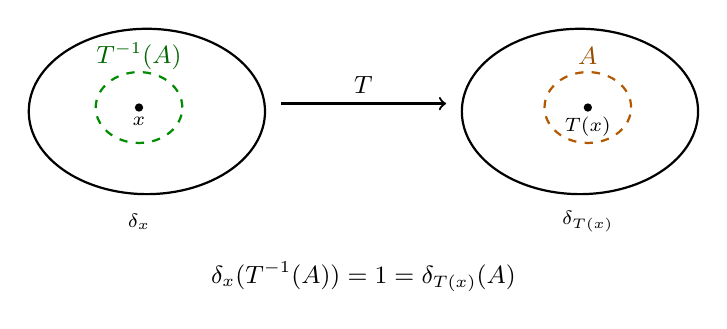
\begin{tikzpicture}[scale=1.0]
  % 左：X 側の楕円と点 x, 囲み T^{-1}(A)
  \draw[thick] (0, 0) ellipse (1.5cm and 1.05cm);
  \node[above right, font=\scriptsize, gray] at (-1.3, 0.7) {$\X$};
  \draw[dashed, thick, green!55!black]
    (-0.1, 0.05) ellipse (0.55cm and 0.45cm);
  \node[font=\small, green!40!black] at (-0.1, 0.7) {$T^{-1}(A)$};
  \fill (-0.1, 0.05) circle (1.5pt) node[below, font=\scriptsize] {$x$};

  % 矢印 T
  \draw[->, thick] (1.7, 0.1) -- (3.8, 0.1)
    node[midway, above, font=\small] {$T$};

  % 右：Y 側の楕円と点 T(x), 囲み A
  \begin{scope}[xshift=5.5cm]
    \draw[thick] (0, 0) ellipse (1.5cm and 1.05cm);
    \node[above right, font=\scriptsize, gray] at (-1.3, 0.7) {$\Y$};
    \draw[dashed, thick, orange!70!black]
      (0.1, 0.05) ellipse (0.55cm and 0.45cm);
    \node[font=\small, orange!60!black] at (0.1, 0.7) {$A$};
    \fill (0.1, 0.05) circle (1.5pt) node[below, font=\scriptsize] {$T(x)$};
  \end{scope}

  % 下：Dirac 測度の値
  \node[font=\scriptsize] at (-0.1, -1.4) {$\delta_x$};
  \node[font=\scriptsize] at (5.6, -1.4) {$\delta_{T(x)}$};
  \node[font=\small] at (2.75, -2.1)
    {$\delta_x(T^{-1}(A)) = 1 = \delta_{T(x)}(A)$};
\end{tikzpicture}
\end{center}

%% ============================================================
%% 凸解析
%% ============================================================
\section{線形代数}
\label{sec:sem-linalg}

\begin{definition}{有限集合と濃度}{sem-finite}
  集合 $S$ が\textbf{有限集合}であるとは，ある $n \in \N$ と
  全単射 $f \colon \range{n} \to S$ が存在することをいう
  （ここで $\range{n} \defeq \{1, 2, \ldots, n\}$）．
  この $n$ を $S$ の\textbf{濃度}といい $|S|$ で表す．
\end{definition}

\begin{claim}{有限集合の最小元}{sem-finite-min}
  $\R$ の空でない有限部分集合 $S$（定義~\ref{def:sem-finite}）には
  最小元が存在する：
  \[
    \exists\, s^* \in S \;\;\text{s.t.}\;\; \forall\, s \in S,\; s^* \leq s.
  \]
\end{claim}

\begin{proof}
  $|S|$ に関する帰納法で示す．

  \textbf{$|S| = 1$ の時．} $S$ の唯一の元がそのまま最小元．

  \textbf{$|S| \geq 2$ の時．}
  $\R$ の任意の空でない有限部分集合 $T$ について $|T| < |S|$ ならば最小元を持つと仮定する．
  $a \in S$ を任意に取り $S' \defeq S \setminus \{a\}$ とおくと $|S'| = |S| - 1$ なので，
  仮定が $S'$ に対して適用でき最小元 $b \in S'$ を持つ．
  $a, b \in \R$ より $b \leq a$ か $a < b$ のいずれかが成り立つので，
  \[
    s^* \defeq
    \begin{cases}
      b & (b \leq a), \\
      a & (a < b)
    \end{cases}
  \]
  とおけば $s^* \in S$ かつ任意の $s \in S$ について $s^* \leq s$．
\end{proof}

\begin{definition}{置換}{sem-permutation}
  $n \in \N$ について，全単射
  $\sigma \colon \range{n} \to \range{n}$ を $\range{n}$ 上の\textbf{置換}という．
  置換全体の集合を
  \[
    \Perm(n) \defeq \{\sigma \colon \range{n} \to \range{n} \mid \sigma \text{ は全単射}\}
  \]
  で表す．$\Perm(n)$ は $|\Perm(n)| = n!$ の有限集合
  （定義~\ref{def:sem-finite}）である．
\end{definition}

\begin{definition}{線形関数}{sem-linear-function}
  ベクトル空間 $V$ から $\R$ への関数 $f \colon V \to \R$ が
  \textbf{線形関数}であるとは，
  任意の $v_1, v_2 \in V$ と $\lambda \in \R$ に対して
  \begin{enumerate}
    \item[(i)] 加法性：$f(v_1 + v_2) = f(v_1) + f(v_2)$，
    \item[(ii)] 斉次性：$f(\lambda v_1) = \lambda f(v_1)$
  \end{enumerate}
  が成り立つことをいう．
\end{definition}

\begin{definition}{全成分 $1$ のベクトル}{sem-ones-vector}
  $n \in \N$ に対し，$\R^n$ の全成分が $1$ のベクトルを
  \[
    \ones_n \defeq (1, 1, \ldots, 1)^\top \in \R^n
  \]
  で表す．
\end{definition}

\begin{definition}{フロベニウス内積}{sem-frobenius-inner}
  同じサイズの2つの行列 $\mathbf{A}, \mathbf{B} \in \R^{n \times m}$ に対し，
  \textbf{フロベニウス内積}を
  \[
    \inner{\mathbf{A}}{\mathbf{B}}
    \defeq \tr(\mathbf{A}^\top \mathbf{B})
    = \sum_{i=1}^{n} \sum_{j=1}^{m} A_{i,j} B_{i,j}
  \]
  で定める．
\end{definition}

\begin{definition}{凸集合}{sem-convex}
  ベクトル空間 $V$ の部分集合 $S \subset V$ が\textbf{凸}であるとは，
  任意の $v_1, v_2 \in S$ と任意の $t \in [0,1]$ に対して
  \[
    t v_1 + (1-t) v_2 \in S
  \]
  が成り立つことをいう．
\end{definition}

\begin{definition}{凸関数と狭義凸関数}{sem-convex-function}
  凸集合 $S \subset V$ 上の関数 $f \colon S \to \R$ が
  \textbf{凸関数}であるとは，任意の $v_1, v_2 \in S$ と
  任意の $t \in [0,1]$ に対して
  \[
    f\bigl(t v_1 + (1-t)v_2\bigr)
    \leq
    t f(v_1) + (1-t) f(v_2)
  \]
  が成り立つことをいう．さらに，任意の相異なる
  $v_1 \neq v_2$ と任意の $t \in (0,1)$ に対して
  \[
    f\bigl(t v_1 + (1-t)v_2\bigr)
    <
    t f(v_1) + (1-t) f(v_2)
  \]
  が成り立つとき，$f$ は\textbf{狭義凸関数}であるという．
\end{definition}
